
\documentclass[12pt]{amsart}
\usepackage{amsmath,amsfonts,amssymb}
\usepackage{algorithm}
\usepackage{pifont}
\usepackage{algpseudocode}
\usepackage{caption}
\usepackage{enumerate}
\usepackage{float}
\usepackage[margin=1in]{geometry}
\usepackage{graphicx}
\usepackage{parskip}
\usepackage{subcaption}
\usepackage{tikz}
\usepackage{tcolorbox}
\tcbuselibrary{skins, breakable}
\usepackage{fancyhdr}
\usepackage{hyperref}
\usepackage{listings}% http://ctan.org/pkg/listings
\lstset{
	basicstyle=\ttfamily,
	language=Python,
	showstringspaces=false,
	mathescape
}
\usepackage{blkarray}
\newcommand{\matindex}[1]{\mbox{\scriptsize#1}}% Matrix index

\theoremstyle{plain}
\newtheorem{theorem}{Theorem}[section]
\newtheorem{corollary}[theorem]{Corollary}
\newtheorem{lemma}[theorem]{Lemma}
\newtheorem{proposition}[theorem]{Proposition}

\theoremstyle{definition}
\newtheorem{definition}[theorem]{Definition}
\newtheorem{example}[theorem]{Example}
\newtheorem{conjecture}[theorem]{Conjecture}
\newtheorem{question}[theorem]{Question}
\theoremstyle{remark}
\newtheorem{remark}[theorem]{Remark}

\newcommand{\cF}{\mathcal F}
\newcommand{\cD}{\mathcal D}
\newcommand{\cP}{\mathcal P}
\newcommand{\cR}{\mathcal R}
\newcommand{\cS}{\mathcal S}
\newcommand{\fS}{\mathfrak S}
\newcommand{\R}{\mathbb{R}}
\newcommand{\dist}{\text{dist}}
\newcommand{\pf}{\text{pf}}
\newcommand{\PP}{\text{P}}
\newcommand{\NP}{\text{NP}}
\newcommand{\Z}{\mathbb{Z}}
\newcommand{\ord}{\text{ord}}
\newcommand{\OPT}{\text{OPT}}
\newcommand{\cost}{\text{cost}}
\newcommand{\price}{\text{price}}
\newcommand{\E}{\text{E}}

\tcbset{breakable, enhanced jigsaw, parbox=false, title=Solution.}

% Header ---------------------------------------------------------------------------
\lhead{CS 8803GA}
\chead{Homework 7 Practice Solutions}
\rhead{\today}
% ----------------------------------------------------------------------------------

\begin{document}
	\thispagestyle{fancy}
	\pagestyle{plain}
	
	\noindent{\bf Problem 1: DPV 7.1} \\
	Consider the following linear program:
	
	\begin{center}
		maximize $5x+3y$\\
		$\begin{aligned}
			5x-2y &\geq 0\\
			x+y &\leq 7\\
			x &\leq 5\\
			x &\geq 0\\
			y &\geq 0\\
		\end{aligned}$
	\end{center}

	Plot the feasible region and identify the optimal solution.
	
	Can you use the dual LP to prove it's optimal?
	
	\begin{tcolorbox}
		\begin{center}
			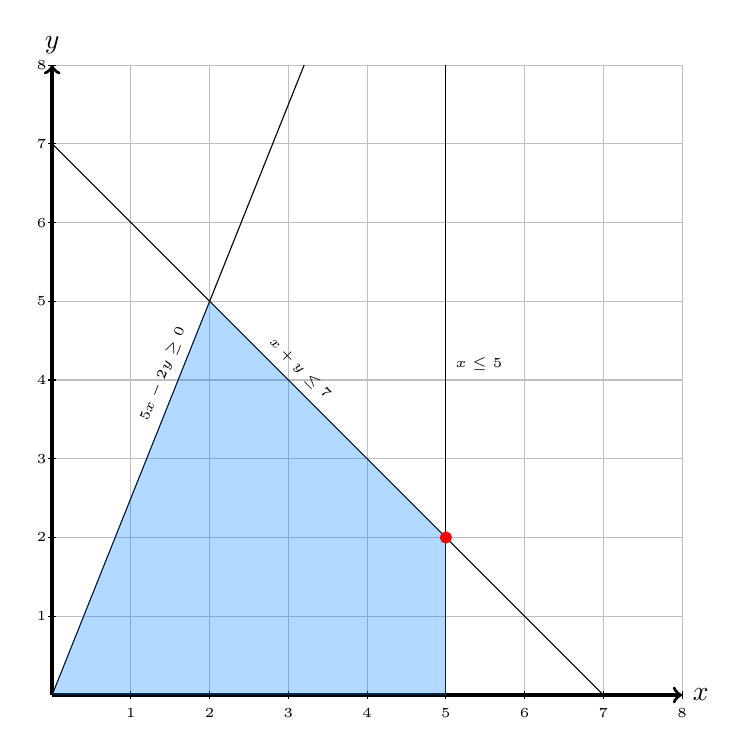
\begin{tikzpicture}[scale=1, every node/.style={scale=1}]
				\draw[gray!50, thin, step=1] (0,0) grid (8,8);
				\draw[very thick,->] (0,0) -- (8,0) node[right] {$x$};
				\draw[very thick,->] (0,0) -- (0,8) node[above] {$y$};
				
				\foreach \x in {1,...,8} \draw (\x,0.05) -- (\x,-0.05) node[below] {\tiny\x};
				\foreach \y in {1,...,8} \draw (-0.05,\y) -- (0.05,\y) node[left] {\tiny\y};
				
				\draw (0,7) -- node[above,sloped] {\tiny$x+y \leq 7$} (6,1) -- (7,0);
				\draw (0,0) -- node[above,sloped] {\tiny$5x - 2y \geq 0$} (3.2,8);
				\draw (5,8) -- node[above right] {\tiny$x \leq 5$} (5,0);
				
				\fill[blue!50!cyan,opacity=0.3] (0,0) -- (2,5)-- (5,2) -- (5,0) -- cycle;
				
				\node[fill,draw,circle,color=red,minimum size=4pt,inner sep=0pt] at (5,2) {};
			\end{tikzpicture}
		\end{center}
	
		The optimal solution is $(5,2)$, with objective value 31.
	
		The dual of this program is
		
		\begin{center}
			minimize $7b+5c$\\
			$\begin{aligned}
			-5a+b+c &\geq 5\\
			2a+b &\geq 3\\
			a &\leq 0\\
			b,c &\geq 0\\
			\end{aligned}$
		\end{center}
		
		We can find a feasible solution for the dual $(0,3,2)$ which has objective value 31.  Since this has the same value as a primal feasible solution (5,2), by weak duality, we can conclude that each of these solutions are optimal for their respective programs.
	\end{tcolorbox}

	\newpage
	\noindent{\bf Problem 2: DPV 7.4 Duff Beer} \\
	Moe is deciding how much Regular Duff beer and how much Duff Strong beer to order each week.  Regular Duff costs Moe \$1 per pint and he sells it at \$2 per pint; Duff Strong cost Moe \$1.50 per pint and he sells it at \$3 per pint.  However, as part of a complicated marketing scam, the Duff company will only sell a pint of Duff Strong for each two pints or more of Regular Duff that Moe buys.  Furthermore, due to past events that are better left untold, Duff will not sell Moe more than 3,000 pints per week.  Moe knows that he can sell however much beer he has.  Formulate a linear program for deciding how much Regular Duff and how much Duff Strong to buy, so as to maximize Moe's profit.  Solve the program geometrically.
	
	\begin{tcolorbox}
		Let $x, y$ be the number of units of Regular and Strong Duff beer respectively that Moe buys.  \\	
		According to the problem description, we can convert the problem into the following LP:
		\begin{equation} \nonumber
		\begin{split}
		\max x & + 1.5y \\
		2y - x & \leq 0 \\
		x + y & \leq 3000 \\
		x, y & \geq 0
		\end{split}
		\end{equation}
		
		\begin{center}
			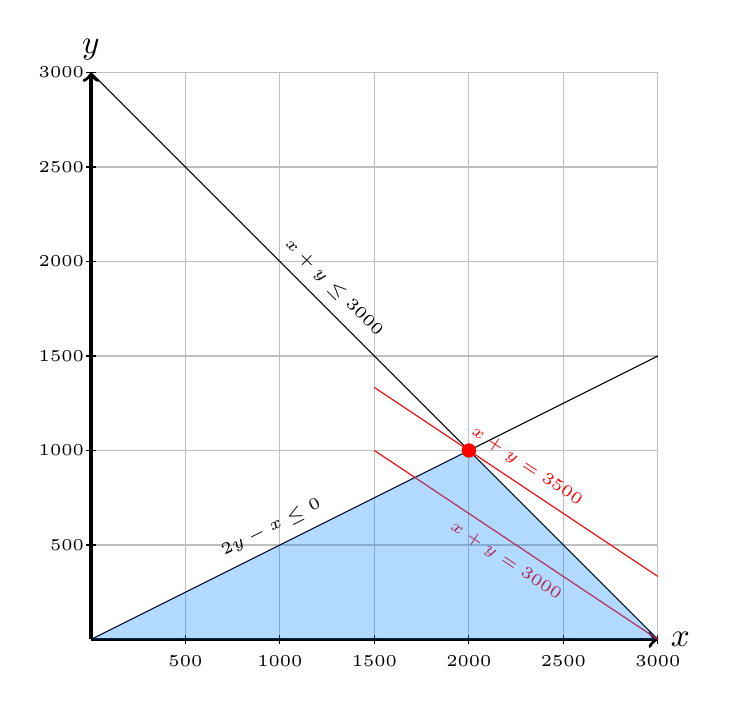
\begin{tikzpicture}[scale=1.2, every node/.style={scale=1.2}]
				\draw[gray!50, thin, step=1] (0,0) grid (6,6);
				\draw[very thick,->] (0,0) -- (6,0) node[right] {$x$};
				\draw[very thick,->] (0,0) -- (0,6) node[above] {$y$};
				
				\foreach \x in {5,10,...,30} \draw (\x/5,0.05) -- (\x/5,-0.05) node[below] {\tiny\x 00};
				\foreach \y in {5,10,...,30} \draw (-0.05,\y/5) -- (0.05,\y/5) node[left] {\tiny\y 00};
				
				\draw (0,0) -- node[above,sloped] {\tiny$2y-x\leq0$} (4,2) -- (6,3);
				\draw (0,6) -- node[above left,sloped] {\tiny$x+y\leq3000$} (6,0);
				
				\draw[red] (3,2.667) -- node[above,sloped] {\tiny$x+y=3500$} (6,0.667);
				\draw[red] (3,2) -- node[below,sloped] {\tiny$x+y=3000$} (6,0);
				
				\fill[blue!50!cyan,opacity=0.3] (0,0) -- (4,2) -- (6,0) -- cycle;
				
				\node[fill,draw,circle,color=red,minimum size=4pt,inner sep=0pt] at (4,2) {};
			\end{tikzpicture}
		\end{center}
		
		The feasible region is shaded and the red lines are equivalent-profit lines. As we can see, $(x, y) = (2000, 1000)$ makes the max profit as \$3,500 for Moe.
	\end{tcolorbox}
	
	\newpage
	\noindent{\bf Problem 3: DPV 7.5 Canine Products} \\
	The Canine Products company offers two dog foods, Frisky Pup and Husky Hound, that are made from a blend of cereal and meat.  A package of Frisky Pup requires 1 pound of cereal and 1.5 pounds of meat, and sells for \$7.  A package of Husky Hound uses 2 pounds of cereal and 1 pound of meat, and sells for \$6.  Raw cereal costs \$1 per pound and raw meat costs \$2 per pound.  It also costs \$1.40 to package the Frisky Pup and \$0.60 to package the Husky Hound.  A total of 240,000 pounds of cereal and 180,000 pounds of meat are available each month.  The only production bottleneck is that the factory can only package 110,000 bags of Frisky Pup per month.  Needless to say, management would like to maximize profit.
	
	(a) Formulate the problem as a linear program in two variables.
	
	\begin{tcolorbox}
		Let $x, y$ be the number of units of Frisky Pup and Husky Hound food respectively made by Canine.\\
		According to the problem description:\\
		the pure profit for a unit of Frisky Pup dog food is 
		\[  \$7 - \$1 \times 1  - \$2 \times 1.5 - \$1.4 = \$1.6;  \]
		the pure profit for a unit of Husky Hound dog food is 
		\[  \$6 - \$1 \times 2  - \$2 \times 1 - \$0.6 = \$1.4.  \]
		Thus, we can convert the problem into the following LP:
		\begin{equation} \nonumber
		\begin{split}
		\max 1.6x & + 1.4y \\
		x + 2y & \leq 240,000 \\
		1.5x + y & \leq 180,000 \\
		x & \leq 110,000 \\
		x, y & \geq 0
		\end{split}
		\end{equation}
	\end{tcolorbox}

	\newpage
	(b) Graph the feasible region, give the coordinates of every vertex, and circle the vertex maximizing profit.  What is the maximum profit possible?
	
	\begin{tcolorbox}
		\begin{center}
			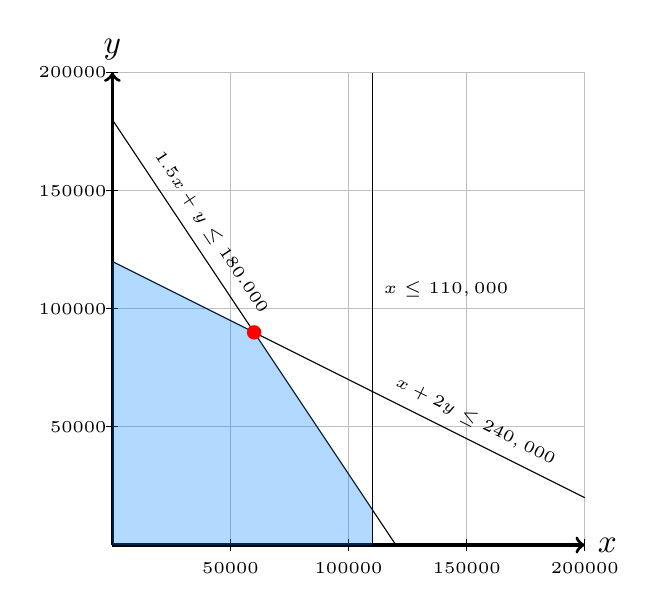
\begin{tikzpicture}[scale=1.5, every node/.style={scale=1.2}]
			\draw[gray!50, thin, step=1] (0,0) grid (4,4);
			\draw[very thick,->] (0,0) -- (4,0) node[right] {$x$};
			\draw[very thick,->] (0,0) -- (0,4) node[above] {$y$};
			
			\foreach \x in {5,10,...,20} \draw (\x/5,0.05) -- (\x/5,-0.05) node[below] {\tiny\x 0000};
			\foreach \y in {5,10,...,20} \draw (-0.05,\y/5) -- (0.05,\y/5) node[left] {\tiny\y 0000};
			
			\draw (0,2.4) -- (2,1.4) -- node[above,sloped] {\tiny$x+2y\leq240,000$} (4,0.4);
			\draw (2.2,4) -- node[above right] {\tiny$x\leq110,000$} (2.2,0);
			\draw (0,3.6) -- node[above left,sloped] {\tiny$1.5x+y\leq180.000$} (2.4,0);
			
			\fill[blue!50!cyan,opacity=0.3] (0,0) -- (0,2.4) -- (1.2,1.8) -- (2.2,0.3) -- (2.2,0) -- cycle;
			
			\node[fill,draw,circle,color=red,minimum size=4pt,inner sep=0pt] at (1.2,1.8) {};
			\end{tikzpicture}
		\end{center}
		
		The feasible region is shaded.
		
		The vertices of the feasible region:\\
		$v_0 = (0, 0), v_1 = (0, 120000), v_2 = (60000, 90000), v_3 = (110000, 15000), v_4=(110000, 0)$\\
		The vertex $v_2 = (60000, 90000)$ makes the max profit as \$222,000 (marked as red).
	\end{tcolorbox}
	
	\newpage
	\noindent{\bf Problem 4: DPV 7.6}  \\
	Give an example of a linear program in two variables whose feasible region is infinite, but such that there is an optimum solution of bounded cost.
	
	\begin{tcolorbox}
		\begin{equation} \nonumber
		\begin{split}
		\max x & - y \\
		x & \leq 1 \\
		x, y & \geq 0
		\end{split}
		\end{equation}
		The feasible region is infinite since we can choose $y$ arbitrarily large. But the target function is bounded above as: $x-y \leq 1$ and equality exists when $(x,y) = (1, 0)$ 
	\end{tcolorbox}

	\newpage
	\noindent{\bf Problem 5: DPV 7.11}  \\
	Write the dual to the following linear program:
	
	\begin{center}
		max $x+y$\\
		$\begin{aligned}
		2x+y &\leq 3\\
		x+3y &\leq 5\\
		x,y &\geq 0\\
		\end{aligned}$
	\end{center}

	Find the optimal solutions to both primal and dual LPs.
	
	\begin{tcolorbox}
		The dual LP is 
		\begin{equation} \nonumber
		\begin{split}
		\min 3z & + 5w\\
		2z + w & \geq 1\\
		z + 3w & \geq 1\\
		z, w & \geq 0.
		\end{split}
		\end{equation}
		The optimal solution of the primal LP is 
		\[(x,y) = ({4}/{5}, {7}/{5}).\]
		The optimal solution of the dual LP is 
		\[ (z,w) = ({2}/{5}, {1}/{5}).\]
		Notice that the optimal values match:
		\[x + y = 3z  + 5w = {11}/{5}.\]
	\end{tcolorbox}

	\newpage
	\noindent{\bf Problem 6: DPV 7.12}  \\
	For the linear program
	
	\begin{center}
		max $x_1-2x_3$\\
		$\begin{aligned}
		x_1-x_2 &\leq 1\\
		2x_2 - x_3 &\leq 1\\
		x_1,x_2,x_3 &\geq 0\\
		\end{aligned}$
	\end{center}

	prove that the solution $(x_1,x_2,x_3)=(3/2, 1/2, 0)$ is optimal.
	
	\begin{tcolorbox}
		The dual LP is 
		\begin{equation} \nonumber
		\begin{split}
		\min y_1 & + y_2\\
		y_1  & \geq 1\\
		-y_1 + 2 y_2 & \geq 0\\
		-y_2 & \geq -2 \\
		y_1, y_2 & \geq 0.
		\end{split}
		\end{equation}
		The dual objective value of the feasible solution $(y_1,y_2) = (1,1/2)$ is 3/2. Since the primal solution $(x_1, x_2, x_3) = (3/2, 1/2, 0)$ is feasible and has the same objective value, it must be optimal.
	\end{tcolorbox}
	
\end{document}







